\documentclass[tikz,border=8pt]{standalone}
% Shared look for every TikZ diagram. Load with \input{../../tools/tikz-style.tex}
\usepackage[sfdefault]{roboto}
\usetikzlibrary{arrows.meta, positioning, shapes.geometric, calc, fit, backgrounds}
\definecolor{cblue}{HTML}{4C78A8}
\definecolor{corange}{HTML}{F58518}
\definecolor{cgreen}{HTML}{54A24B}
\definecolor{cred}{HTML}{E45756}
\definecolor{cpurple}{HTML}{B279A2}
\definecolor{cgrey}{HTML}{6B6B6B}
\tikzset{
  every picture/.style={font=\sffamily, line width=1.2pt},
  box/.style={draw=#1, fill=#1!12, rounded corners=4pt, align=center, inner sep=7pt, minimum height=1.1cm},
  box/.default=cgrey,
  arrow/.style={-{Stealth[length=3mm]}, draw=cgrey, line width=1.4pt},
  title/.style={font=\sffamily\bfseries\Large},
  note/.style={font=\sffamily\small, text=cgrey, align=center},
}
\AtBeginDocument{\hyphenpenalty=10000 \exhyphenpenalty=10000}

% Apollo master (modules/planning): routing A* on the lane graph; reference line 180-250 m ahead, smoothed by the
% FEM-position-deviation QP (OSQP) every 50 ms; lane_follow pipeline: piecewise-jerk path QP (0.5 m over 100 m),
% DP speed on the station-time grid, piecewise-jerk speed QP (0.1 s over 7 s); 8 s trajectory per prediction message.
% Open space: Hybrid A* warm start, iterative anchoring smoother, piecewise-jerk speed QP.
\begin{document}
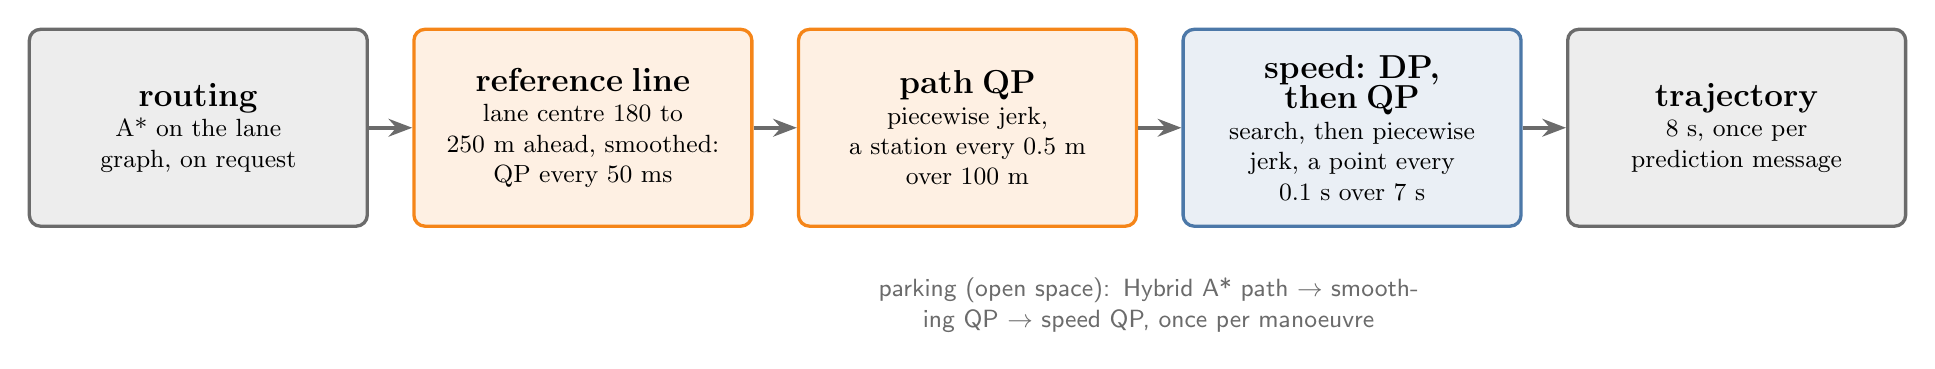
\begin{tikzpicture}[node distance=0.55cm,
  st/.style={box=#1, font=\small, minimum width=4.1cm, text width=3.8cm, minimum height=2.5cm}]
  \node[st=cgrey] (a) {{\large\textbf{routing}}\\ A* on the lane\\ graph, on request};
  \node[st=corange, right=of a] (b) {{\large\textbf{reference line}}\\ lane centre 180 to\\ 250 m ahead, smoothed:\\ QP every 50 ms};
  \node[st=corange, right=of b] (c) {{\large\textbf{path QP}}\\ piecewise jerk,\\ a station every 0.5 m\\ over 100 m};
  \node[st=cblue, right=of c] (d) {{\large\textbf{speed: DP, then QP}}\\ search, then piecewise\\ jerk, a point every\\ 0.1 s over 7 s};
  \node[st=cgrey, right=of d] (e) {{\large\textbf{trajectory}}\\ 8 s, once per\\ prediction message};
  \draw[arrow] (a) -- (b); \draw[arrow] (b) -- (c); \draw[arrow] (c) -- (d); \draw[arrow] (d) -- (e);
  \node[note, below=0.5cm of c, xshift=2.3cm, text width=12cm] {parking (open space): Hybrid A* path $\rightarrow$ smoothing QP $\rightarrow$ speed QP, once per manoeuvre};
\end{tikzpicture}
\end{document}
